\section{Background on the Heart }
\begin{figure*}[htbp]
	\centering
	{
	\centering
	\subfigure[\label{fig:heart} Diagram of the heart. Reproduced 
	from~\cite{zhihao12}]{
       \framebox[0.31\textwidth]{
				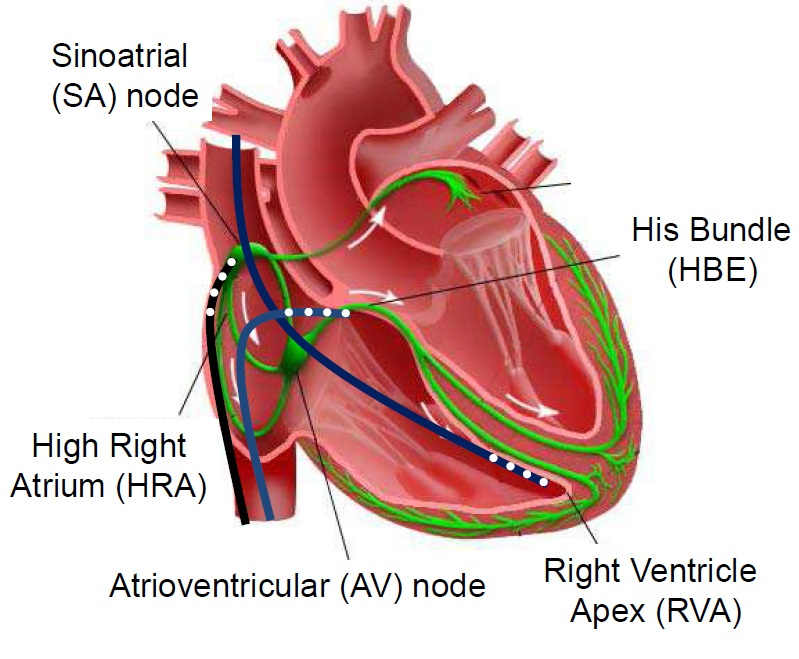
\includegraphics[width=0.262\linewidth]{figures/heart}
		} %framebox
	}
	\subfigure[The four stages of an \acf{AP}]{
		\framebox[0.31\textwidth]{
			\begin{tikzpicture}[transform shape, xscale=0.6, yscale=0.6]
\begin{axis}
[ xlabel={Time (ms)},
ylabel={Potential ({mV})},
axis y line = left,
axis x line = bottom,
xmin=0,   xmax=300,
ymin=0,   ymax=150,
ytick={0, 30, 44.5, 50, 100, 131.1, 150},
yticklabels={0, $v_R$, $v_T$, 50, 100, $v_O$, 150},
extra tick style={grid=major}
]
\addplot[color=blue!90,
mark=.,
mark size=2,
smooth,
const plot
]
table [x=t, y=v, col sep=comma] {./figures/actionPotentialData.csv};

\addplot[color=black!90,
dashed,
mark=.,
mark size=2
] coordinates {
	(0,30)
	(240,30)
};

\addplot[color=black!90,
dashed,
mark=.,
mark size=2
] coordinates {
	(0,44.5)
	(50,44.5)
};

\addplot[color=black!90,
dashed,
mark=.,
mark size=2
] coordinates {
	(0,131.1)
	(50,131.1)
};

\end{axis}

\tikzstyle{every state}=[rectangle, text centered, draw=none,text=black, draw,line width=0.3mm]

\node[state, shift={(0.2, -1.5)}, fill=green!20, inner xsep=0.0cm, minimum width=0.6cm] {RP};
\node[state, shift={(0.85, -1.5)}, fill=yellow!20, minimum width=0.5cm] {ST};
\node[state, shift={(3.00, -1.5)}, fill=red!20, minimum width=2.8cm] {ERP};
\node[state, shift={(1.50, -1.5)}, fill=blue!20, minimum width=0.5cm] {UP};
\node[state, shift={(5.15, -1.5)}, fill=green!20, minimum width=1.5cm] {RRP};
\node[state, shift={(6.40, -1.5)}, fill=green!20, minimum width=1cm] {RP};

\end{tikzpicture}
			\label{fig:actionPotential}
		}
	}
	\subfigure[An abstracted model of the conduction system]{ 
          \framebox[0.31\textwidth]{
          	\begin{tikzpicture}[->,>=stealth',semithick,scale=0.73, transform shape]

\tikzstyle{every state}=[fill=blue!20,circle,minimum size=0.1cm]

\tikzset{
	atrialCell/.style={
		fill=green!20,
		circle,
		minimum size=0.1cm,
		draw,
		line width=0.2mm
	}
}

\tikzset{
	ventricularCell/.style={
		fill=blue!20,
		circle,
		minimum size=0.1cm,
		draw,
		line width=0.2mm
	}
}

\tikzset{
	autorhythmicCell/.style={
		fill=yellow!20,
		circle,
		minimum size=0.1cm,
		draw,
		line width=0.2mm
	}
}

\draw node[atrialCell](SA) {\footnotesize SA};

\node[atrialCell](CT) [below left=0.3cm and 0.5cm of SA] {};
\node[atrialCell](CT1) [below left=0.5cm and 0cm of CT] {};

\node[atrialCell](BB) [below right=-0.1cm and 0.5cm of SA] {};
\node[atrialCell](LA) [below right=-0.1cm and 0.5cm of BB] {};
\node[atrialCell](LA1) [below right=-0.1cm and 0.5cm of LA] {};

\node[atrialCell](RA) [below left=0.4cm and -0.1cm of SA] {};
\node[atrialCell](RA1) [below left=0.5cm and 0cm of RA] {};
\node[atrialCell](CS) [below left=0.5cm and -0.3cm of RA1] {};

\node[atrialCell](OS) [below right=0.4cm and 0.2cm of SA] {};
\node[atrialCell](Fast) [below left=0.4cm and -0.1cm of OS] {};
\node[atrialCell](Fast1) [below right=0.4cm and -0.1cm of Fast] {};
\node[atrialCell](Slow) [below right=0.2cm and 0.3cm of OS] {};
\node[atrialCell](Slow1) [below right=0.4cm and -0.1cm of Slow] {};
\node[atrialCell](AV) [below right=0.2cm and 0.3cm of Fast1] {\footnotesize AV};

\node[ventricularCell](His) [right=0.3cm of AV] {};
\node[ventricularCell](His1) [below right=-0.1cm and 0.3cm of His] {};
\node[ventricularCell](His2) [below right=0.3cm and -0.1cm of His1] {};

\node[ventricularCell](RBB) [below left=0.4cm and 0.1cm of His2] {};
\node[ventricularCell](RBB1) [below right=0.4cm and -0.1cm of RBB] {};
\node[ventricularCell](RVA) [below right=0.4cm and -0.1cm of RBB1] {};

\node[ventricularCell](LBB) [below right=0.4cm and 0.2cm of His2] {};
\node[ventricularCell](LBB1) [below right=0.4cm and -0.1cm of LBB] {};
\node[ventricularCell](LVA) [below right=0.4cm and -0.1cm of LBB1] {};

\node[ventricularCell](LVS) [above right=0.3cm and 0.3cm of LVA] {};
\node[ventricularCell](LVS1) [above left=0.4cm and -0.1cm of LVS] {};
\node[ventricularCell](CSLV) [above left=0.4cm and -0.1cm of LVS1] {};

\node[ventricularCell](LV) [above right=0.1cm and 1.0cm of LVA] {};
\node[ventricularCell](LV1) [above left=1.8cm and -0.1cm of LV] {};

\node[ventricularCell](RVS) [above left=0.2cm and 0.6cm of RVA] {};
\node[ventricularCell](RVS1) [above left=0.4cm and -0.1cm of RVS] {};

\node[ventricularCell](RV) [above left=-0.1cm and 1.2cm of RVA] {};
\node[ventricularCell](RV1) [above left=0.9cm and 0.8cm of RV] {};

\path[-] (SA) edge (BB);
\path[-] (BB) edge (LA);
\path[-] (LA) edge (LA1);

\path[-] (SA) edge (CT);
\path[-] (CT) edge (CT1);

\path[-] (SA) edge (RA);
\path[-] (RA) edge (RA1);
\path[-] (RA1) edge (CS);

\path[-] (SA) edge (OS);
\path[-] (OS) edge (Fast);
\path[-] (Fast) edge (Fast1);
\path[-] (OS) edge (Slow);
\path[-] (Slow) edge (Slow1);
\path[-] (Fast1) edge (AV);
\path[-] (Slow1) edge (AV);

\path[-] (AV) edge (His);
\path[-] (His) edge (His1);
\path[-] (His1) edge (His2);
\path[-] (His2) edge (RBB);
\path[-] (RBB) edge (RBB1);
\path[-] (RBB1) edge (RVA);
\path[-] (His2) edge (LBB);
\path[-] (LBB) edge (LBB1);
\path[-] (LBB1) edge (LVA);
\path[-] (RVA) edge (LVA);

\path[-] (RVA) edge (RVS);
\path[-] (RVS) edge (RVS1);

\path[-] (RVA) edge (RV);
\path[-] (RV) edge (RV1);

\path[-] (LVA) edge (LVS);
\path[-] (LVS) edge (LVS1);
\path[-] (LVS1) edge (CSLV);

\path[-] (LVA) edge (LV);
\path[-] (LV) edge (LV1);

\end{tikzpicture}
          	\label{fig:heartNetwork} 
	  } %framebox
	}

}
	\caption{Electrical conduction systems of the heart}
	\label{fig:heartOverview}
\end{figure*}

In this section, using Figure~\ref{fig:heartOverview} we 
describe the electrical conduction system of the heart.\\

\noindent \textbf{Heart.}
The human heart (see Figure~\ref{fig:heart})
 is an organ that pumps blood throughout the body.
It achieves this by regularly contracting and relaxing the muscles
which are orchestrated by a flow of electrical signals through the heart.
The signal is primarily generated automatically by the \ac{SA} node.
First, the signal travels through the left and right atria, contracting 
the muscles and pushing the blood into the ventricles.
 
Second, to ensure both ventricles are filled, 
the \ac{AV} node introduces critical delay 
in the conduction system.   
Finally, the electrical signal propagates through 
both ventricles. This contracts the muscles and pumps the blood out of the heart.
\\

\noindent \textbf{\acf{AP}.} 
The propagation of electrical signals at a cellular level 
is described as a change in  voltage 
across the cell membrane due to ionic flow. Over a period of time, 
this change is known as an \acf{AP}~\cite{chen14} as shown in Figure~\ref{fig:actionPotential}. 
The \ac{AP} can be described in four stages.
\begin{enumerate}
	\item \acf{RP}: This is the steady state of the cell while awaiting 
					activation by an external stimulus.
	\item \acf{UP}: When activated by an external stimulus, 
					the cell depolarises (inward flow of positive ions) and 
					contracts the muscles. This depolarisation yields 
					a stimulus that activates neighbouring cells.
	\item \acf{ERP}: Once activated, the cell cannot be activated again 
					 due to the recovery process of the ionic channels. 
					 Any new stimulus will be blocked. 
	\item \acf{RRP}: During this period, the ionic channels are partially recovered
					 and the cell can be activated. However, the morphology
					 of the \ac{AP} will be shorter.\\
	
\end{enumerate}


\noindent \textbf{Abstract model.}
The human heart has over two trillion cells. For analytical purposes, a
model consisting of a network of $32$ nodes is presented in literature
and is used for testing off-the-shelf pacemakers~\cite{chen14,zhihao12}.
The abstracted electrical conduction system consisting  of 
nodes and paths is presented in Figure~\ref{fig:heartNetwork}.
The functionality of each node is described using \acf{HA} in Section~\ref{sec:HA}. The path model describes the 
conduction delay of the electrical signal.
Later in Section~\ref{sec:codeGen}, we use the abstract network model 
to illustrate our modular code generation.

 
